\documentclass[5p,times]{elsarticle}

\usepackage[a4paper, margin=1.37in]{geometry}
\usepackage[english]{babel}
\usepackage[utf8]{inputenc}
\usepackage{amsmath}
\usepackage{amsfonts}
\usepackage{amsthm}
\usepackage{amssymb}
\usepackage{fancyhdr}
\usepackage{xifthen}
\usepackage{tabularx,lipsum,environ,amsmath,amssymb}
\usepackage{cite}
\usepackage[T1]{fontenc}
\usepackage{todonotes}
\usepackage{hyperref}
\usepackage{tikz}
\usepackage{aliascnt}
\usepackage{tikz-qtree,tikz-qtree-compat}

\usetikzlibrary{shapes,arrows,matrix,positioning,calc,positioning,automata,shadows,fit}

% Matrix drawing
\newcommand{\msize}{2em}
\tikzstyle{redblock} = [draw, fill=red, rectangle, minimum width=\msize, minimum height=\msize]
\tikzstyle{blueblock} = [draw, fill=blue, rectangle, minimum width=\msize, minimum height=\msize]
\tikzstyle{grayblock} = [draw, fill=gray, rectangle, minimum width=\msize, minimum height=\msize]
\tikzstyle{whiteblock} = [draw, fill=white, rectangle, minimum width=\msize, minimum height=\msize]

\newcommand{\redb}{\node[redblock] {};}
\newcommand{\blueb}{\node[blueblock] {};}
\newcommand{\grayb}{\node[grayblock] {};}
\newcommand{\whiteb}{\node[whiteblock] {};}
	
%	\begin{tikzpicture}
%	\matrix[matrix of nodes] {
%		\redb  &\redb  &\whiteb&\whiteb\\
%		\redb  &\redb  &\whiteb&\blueb \\
%		\whiteb&\whiteb&\blueb &\blueb \\
%		\whiteb&\whiteb&\blueb &\whiteb\\
%	};
%	\end{tikzpicture}

% NP PROBLEM
\makeatletter
\newcommand{\problemtitle}[1]{\gdef\@problemtitle{#1}}% Store problem title
\newcommand{\probleminput}[1]{\gdef\@probleminput{#1}}% Store problem input
\newcommand{\problemquestion}[1]{\gdef\@problemquestion{#1}}% Store problem question
\NewEnviron{problem}{
  \problemtitle{}\probleminput{}\problemquestion{}% Default input is empty
  \BODY% Parse input
  \par\addvspace{.5\baselineskip}
  \noindent
  \begin{tabularx}{\textwidth}{@{\hspace{\parindent}} l X c}
    \multicolumn{2}{@{\hspace{\parindent}}l}{\textsc{\@problemtitle}} \\% Title
    \textbf{Input:} & \@probleminput \\% Input
    \textbf{Question:} & \@problemquestion% Question
  \end{tabularx}
  \par\addvspace{.5\baselineskip}
}

% THEOREM ENVIRONMENTS
\newtheorem{theorem}{Theorem}[section]

\newaliascnt{lemma}{theorem}
\newtheorem{lemma}[lemma]{Lemma}
\aliascntresetthe{lemma}
\providecommand*{\lemmaautorefname}{Lemma}

\newaliascnt{proposition}{theorem}
\newtheorem{proposition}[proposition]{Proposition}
\aliascntresetthe{proposition}
\providecommand*{\propositionautorefname}{Proposition}

\newaliascnt{corollary}{theorem}
\newtheorem{corollary}[corollary]{Corollary}
\aliascntresetthe{corollary}
\providecommand*{\corollaryautorefname}{Corollary}

\newaliascnt{definition}{theorem}
\newtheorem{definition}[definition]{Definition}
\aliascntresetthe{definition}
\providecommand*{\definitionautorefname}{Definition}

%\newtheorem{lemma}[theorem]{Lemma}
%\newtheorem{proposition}[theorem]{Proposition}
%\newtheorem{corollary}[theorem]{Corollary}
%\newtheorem{definition}[theorem]{Definition}

% NP Complete
\newcommand{\NP}{$\mathcal{NP}$}
\newcommand{\NP}{$\mathcal{P}$}

% Do not split footnotes over multiple pages
\interfootnotelinepenalty=10000



\begin{document}

	\title{An improved exact algorithm and an NP-completeness proof for sparse matrix bipartitioning}

	\author[timon]{Timon E. Knigge\corref{cor}}
	\ead{knigget@student.ethz.ch}
	\address[timon]{ETH Z\"urich\\
				Z\"urich, Switzerland}

	\author[rob]{Rob H. Bisseling}
	\ead{R.H.Bisseling@uu.nl}
	\address[rob]{Mathematical Institute,
				Utrecht University\\
				Utrecht, The Netherlands}

	\cortext[cor]{Corresponding author}

	\begin{abstract}
		We formulate the sparse matrix bipartitioning problem of
		minimizing the communication volume in parallel sparse
		matrix-vector multiplication. We prove its \NP-completeness
		in the perfectly balanced case, where both parts of the
		partitioned matrix must have an equal number of nonzeros,
		by reduction from the graph bisection problem.

		We present an improved exact branch-and-bound algorithm
		which finds the minimum communication volume for a given
		maximum allowed imbalance. The algorithm is based on a
		maximum-flow bound and a packing bound, which extend
		previous matching and packing bounds.

		We implemented the algorithm in a new program called MP
		(Matrix Partitioner), which solved 839 matrices from the
		SuiteSparse collection to optimality, each within 24 hours
		of CPU-time. Furthermore, MP solved the difficult problem
		of the matrix \texttt{cage6} in about 3 days. The new
		program is about 13.8 times faster than the previous program
		MondriaanOpt.
	\end{abstract}
	\begin{keyword}
		Bisection \sep Exact Algorithm \sep Maximum Flow \sep
		NP Complete \sep Partitioning \sep Sparse Matrix
	\end{keyword}

	\maketitle


	\section{Introduction}
\label{sec:intro}
Sparse matrix partitioning is important for the parallel solution of sparse linear systems
by direct or iterative methods. In iterative solvers, the basic kernel is the multiplication
of a sparse matrix and a dense vector, the SpMV operation. A good partitioning of the sparse matrix
and vector will balance the computation load in a parallel SpMV by spreading the
matrix nonzeros evenly over the parts assigned to the processors 
of the parallel computer and it will also
lead to less communication of the vector components between the processors.

In the past decades, much effort has been spent on developing and improving
heuristic partitioning methods. In particular, hypergraph methods have been very
succesful because they model the communication volume (the total
number of data words sent) exactly, so that they can try to minimise the true metric.
Two-dimensional (2D) partitioning methods are superior to 1D methods,
since they are more general and can split both the rows and columns of the matrix and
hence in principle can provide better solutions.
Heuristic algorithms for hypergraph-based sparse matrix partitioning
have been implemented in the sequential software packages hMetis~\cite{karypis99b},
PaToH~\cite{catalyurek99}, Mondriaan~\cite{vastenhouw05}, KaHyPar~\cite{akhremtsev17},
and the parallel packages Par$k$way~\cite{trifunovic08} and Zoltan~\cite{devine06}.
The current state-of-the art methods for 2D sparse matrix partitioning are the fine-grain~\cite{catalyurek01}
and the medium-grain method~\cite{pelt14}. 

How good are the current methods and is it still worthwhile to improve them?
To answer this question we need to compare the quality of the outcome,
i.e., the communication volume, to the optimal result.
To enable such a comparison, we need an exact algorithm that provides the 
minimum communication volume for a specfied maximum load imbalance.
The first exact algorithm for this problem (with two parts)
was proposed by Pelt and Bisseling~\cite{pelt15}.
It is based on a branch-and-bound method that distinguishes  between
three cases for every row and column of the sparse matrix:
completely assigned to part 0, completely assigned to part 1, 
or split between the two parts. This algorithm has been implemented
in the program MondriaanOpt, included in the Mondriaan package,
version 4.2. As of today, 356 matrices from the SuiteSparse 
(formerly University of Florida) sparse matrix collection~\cite{davis11}
have been bipartitioned to optimality by MondriaanOpt. 
\footnote{The solutions can be found at
\url{http://www.staff.science.uu.nl/~bisse101/Mondriaan/Opt/}.}
Being able to increase the size of the solution subset would be valuable
for benchmarking heuristic partioners, by providing more comparison data and also  
for more realistic problem sizes. Heuristic partitioners are aimed at large 
problesm, though they will encounter smaller problems after their inital splits.

Optimal partitionings are easiest to compute for two parts:
the required computation time
grows quickly with a larger number of parts, as discussed in~\cite{pelt15}.
Furthermore, heuristic partitioners often are based on recursive bipartitioning,
so that it is most important to gauge the quality of the bipartitioner.
(A notable exception is KaHyPar, which computes a direct $k$-way partitioning.)
Therefore, both the exact partitioner implemented in MondriaanOpt and the improved partioner 
MP (for Matrix Partitioner)
presented in this article, compute optimal solutions for bipartitioning.

Another question that arises is about the NP-completeness~\cite{garey79}
of the sparse matrix bipartitioning problem.
It is known that the decision problem of
graph bipartitioning with a tolerated imbalance
is NP-complete~\cite[Theorem 3.1]{bui92}
and so is hypergraph partitioning~\cite[Chapter 6]{lengauer90}, 
but sparse matrix bipartitioning is a special
case of hypergraph bipartitioning (with vertices contained in only two hyperedges),
and its decision problem is expected to be NP-complete,
but this has not been proven yet.

The novelty of this paper is twofold: (i) we present an improvement
of the previous exact algorithm from~\cite{pelt15} by generalising
a matching-based lower bound on the necessary communication
to a stronger maximum flow-based bound; (ii) we formulate the balanced sparse matrix bipartitioning problem
and prove its NP-completeness.

The sparse matrix bipartitioning problem that
we solve by an exact algorithm can be formulated as follows.
Given an $m \times n$ sparse matrix with $|A|$ nonzeros
and an allowed imbalance fraction of $\epsilon \geq 0$,
find disjoint subsets $A_0, A_1 \subseteq A$ such that
\begin{equation}
A=A_0 \cup A_1,
\end{equation}
and
\begin{equation}
\label{eqn:imbal}
|A_i| \leq (1+\epsilon ) \left\lceil \frac{|A|}{2} \right\rceil ,
~\mathrm{for}~ i=0,1,
\end{equation}
and such that the communication volume $V(A_0,A_1)$ is minimal.

Here, the \emph{communication volume} is
defined as the total number of rows and columns 
that have nonzeros in both subsets.
Each of these \emph{cut} rows and columns gives rise to one communication
in a parallel SpMV.
Eqn~(\ref{eqn:imbal}) represents a constraint on the load balance
of two processors of a parallel computer executing the SpMV. 

In this paper, we will only consider the communication volume
as the metric to be minimised. 
Note that other possible objectives, such as 
minimising the maximum communication volume per processor
or minimising the total number of messages, 
may also be relevant for a larger numbers of parts,
but not for two parts.

Many exact partitioning algorithms have been developed for graphs~\cite{karisch00,sensen01,felner05,hager13,delling14}. All these algorithms minimise the edge cut,
not the communication volume.
Felner~\cite{felner05} solves a graph partitioning problem
with uniform edge weights to optimality
with a purely combinatorial branch-and-bound method,
reaching up to 100 vertices and 1000 edges.
Delling~\textit{et al.\ }\cite{delling14} solved larger problems
using packing-tree bounds and graph contractions, and they solved 
the open street map problem \texttt{luxembourg} with
114,599 vertices and 119,666 edges in less than a minute.

For hypergraphs, much less work has been
done on exact partitioning~\cite{caldwell00,kucar04,bisseling05}.
Kucar~\cite{kucar04} uses integer linear programming (ILP) 
to solve a problem with 1888 vertices, 1920 nets (hyperedges), and 5471
pins (nonzeros) in three days of CPU time; the heuristic solver
hMetis~\cite{karypis99b}
managed to find a solution in less than a second for the same problem,
and it turned out to be optimal.
Bisseling and his team members~\cite{bisseling05}
solved an industrial call-graph problem
by formulating it as a hypergraph partitioning problem with the cut-net metric,
and they solved it heuristically by using Mondriaan
and exactly by an ILP method (in 9 days of CPU time).

For exact sparse matrix partitioning,
the problem could in principle be formulated
as a hypergraph bipartitioning problem by using
the fine-grain model~\cite{catalyurek01}:
each matrix nonzero becomes a vertex in the hypergraph;
the nonzeros in a row are connected by a row-net  
and the nonzeros in a column by a column-net.
Thus, we obtain a hypergraph with $|A|$ vertices and $m+n$ nets,
with the special property that each vertex is
contained in precisely two nets.
An exact general hypergraph partitioner could then be used to solve
the problem to optimality. 
This, however, is less efficient than direct exact sparse matrix partitioning,
since the hypergraph partitioner would not exploit the special property.
In contrast, the direct matrix approach imposes this property
by construction.

Our previous work~\cite{pelt15} presented the first direct
exact matrix partitioner, implemented in the open-source software
MondriaanOpt. This work was extended by Mumcuyan
and coworkers~\cite{mumcuyan18} who 
reordered the matrix given to MondriaanOpt,
automatically choosing the best reordering method
from a set of methods by a machine-learning approach,
and by parallelising the software for a shared-memory computer
using OpenMP. 
Our own improvements, in the present article,
are orthogonal to these extensions,
so that they can be combined.  

The remainder of this paper is organised as follows:
Section~\ref{sec:np} presents the NP-completeness proof 
for sparse matrix bipartitioning.
Section~\ref{sec:opt} briefly reviews the
branch-and-bound algorithm of~\cite{pelt15}
that was implemented in MondriaanOpt.
Section~\ref{sec:experiments} presents the experimental results,
comparing MP to MondriaanOpt for 233 small matrices, 
and giving results for 599 larger matrices that could not be solved
by MondriaanOpt within the allotted time.
Section~\ref{sec:concl} presents the conclusions and discusses possible future
work.


		\section{Hardness results}
	\label{sec:np}
	In this section we will formally analyze the matrix partitioning
	problem and prove that it is \NP-Complete, even if we fix the
	the number of processors to $k = 2$. We will assume we are looking
	for a perfect partitioning, i.e. with imbalance parameter $\epsilon = 0$.

	\subsection{Preliminaries}
	\label{1-preliminaries}
	To begin, let us define a formal decision-variant of the matrix
	partitioning problem for $k = 2$, based on the optimization
	variant described in \autoref{sec:intro} where the goal
	is to minimize the total communication volume. We formulate our
	decision problems in the style of \cite{garey79}.

	\begin{problem}
		\problemtitle{\mbpt}
		\probleminput{An $m \times n$ matrix $A$, whose nonzeros are precisely
			indexed by the set
			$Z \subseteq \{\, 1, \dots, m \,\} \times
				\{\, 1, \dots, n \,\}$, and an integer $V$, the required
			maximum volume.}
		\problemquestion{Does there exist a disjoint partitioning of $Z$
			into $Z_1 \cup Z_2$ such that $|Z_1| = |Z_2|$ and volume
			$VOL(Z_1, Z_2) \leq V$?}
	\end{problem}

	Here $VOL(Z_1, Z_2)$ counts the number of rows and columns that
	have nonzeros in $Z_1$ and $Z_2$, as before. Note that unlike before,
	we require $|Z_1|$ and $|Z_2|$ to be exactly equal, which implicitly
	requires that the number of nonzeros is even. This is not a very big
	problem however: if $|Z|$ is odd, we can add one more dummy row and column
	with a single nonzero. Then we can proceed under the assumption that $|Z|$
	is even and at least one equipartitioning exists, and remove the dummy
	nonzero at the end again.

	When thinking about the matrix bipartitioning problem, it is helpful
	to reformulate it in terms of graphs. Given an $m \times n$ matrix $A$
	we can define a bipartite adjacency graph $G(A) = (V(A), E(A))$ with
	$m$ vertices representing the rows of $A$, and $n$ vertices representing
	the columns, where a row vertex $r$ and a column vertex $c$ are connected
	if and only if $A_{rc}$ is nonzero.

	This equivalence extends to the partitioning problem. A bipartitioning of
	the nonzeros of $A$ corresponds to a bipartitioning of the edges of $G(A)$,
	and the rows and columns contributing to the final volume correspond
	precisely to the vertices with edges in both sides of the partition. See
	also the figure.

	\begin{figure}[h]
		\begin{tikzpicture}
[
	box/.style={rectangle,draw=black,thick, minimum size=0.5cm},
]
		
	\begin{scope}
		\node at (3.5, 0){\huge$\rightarrow$};
	\end{scope}

	\begin{scope}[shift={(0, 0)}]
		\foreach \x in {0,0.5,1}{
			\foreach \y in {0,0.5,1}
				\node[box] at (\x,\y){};
		}
		\node[box,fill=gray] at (0, 1){};
		\node[box,fill=gray] at (0.5, 1){};
		\node[box,fill=gray] at (1, 0.5){};
		\node[box,fill=gray] at (0.5, 0){};
		\node[] at (-0.5,	0) {3};
		\node[] at (-0.5,	0.5) {2};
		\node[] at (-0.5,	1) {1};
		\node[] at (0,	1.5) {5};
		\node[] at (0.5,	1.5) {6};
		\node[] at (1,	1.5) {7};
	\end{scope}


	\begin{scope}
		\node[shape=circle,fill=white,draw=black,minimum size=13pt] (1) at ($(-0.5,{sqrt(3)*-0.5})$) {1};
		\node[shape=circle,fill=white,draw=black,minimum size=13pt] (2) at ($(-0.5,{sqrt(3)*0.5})$) {2};
		\node[shape=circle,fill=white,draw=black,minimum size=13pt] (3) at (1, 0){3};
		\node[shape=circle,fill=white,draw=black,minimum size=13pt] (4) at ($({1+sqrt(2)}, 0)$) {4};
		
		\draw[line width=1.5pt] (1) -- (2) -- (3) -- (1);
		\draw[line width=1.5pt] (3) -- (4);
	\end{scope}
\end{tikzpicture}

		\centering
		\label{mat-equiv-fig}
		\caption{Graph and matrix equivalence.}
	\end{figure}
	
	It should be clear this procedure is also reversible, i.e. for any
	bipartite graph $G$ on $m$ and $n$ vertices,
	we can construct a corresponding matrix $A$ of size $m \times n$ which has
	nonzeros precisely for the vertices that are connected in $G$. While the
	nonzero entries of this matrix can be any value, the associated nonzero
	pattern is uniquely determined by the edges of $G$.

	To this end we define an equivalent bipartitioning problem on graphs that
	we will base our reduction on:

	\begin{problem}
		\problemtitle{\geb}
		\probleminput{Given a graph
			$G = (V, E)$ and an integer
			$M$.}
		\problemquestion{Does there exist a disjoint partitioning of $E$
			into $E_1 \cup E_2$ such that $|E_1| = |E_2|$ and
			$\big|\big(\bigcup_{e\in E_1} e \big) \cap
				\big(\bigcup_{e\in E_2} e \big)\big| \leq M$?\footnote{
			Writing an edge as the set $\{ u, v\} \subset V$, then
			$\bigcup_{e \in E_1} e$ gives precisely the set of vertices touched
			by $E_1$.}}
	\end{problem}

	We call a vertex with adjacent edges from both partitions `cut'. The
	goal is to minimize the number of cut vertices. Additionally, when we
	explicitly need the partitioning/coloring of $E$, we will write it 
	as a map $\pi : E \to \{0,1\}$.

	\subsection{\geb is \NP-Complete}
	We will perform a reduction from \gb which was proven \NP-Complete in
	\cite{gb-np-complete} under the name \textsc{Minimum \allowbreak
	cut \allowbreak into \allowbreak equal-\allowbreak sized \allowbreak
	subsets}.

	\begin{problem}
		\problemtitle{\gb}
		\probleminput{A graph $G = (V, E)$, an integer $M$.}
		\problemquestion{Does there exist a disjoint partition of $V$
			into $V_1 \cup V_2$ with $|V_1| = |V_2|$ and such that
			$|\{\, \{u, v\} \,\mid\, u \in V_1, v\in V_2 \,\}| \leq M$?}
	\end{problem}

	Analogously to \geb, an edge with endpoints in both sides of the
	partition is called `cut', the goal is to minimize the number of
	cut edges. We similarly write a partitioning of $V$ as
	a map $\tau : V \to \{0, 1\}$. We can also think of $\tau$ as coloring
	the vertices in $V$, where one side of the partition has the color red, and one
	side has the color blue. However this should not be confused with the classical
	graph coloring problem, since we allow neighbouring vertices to have the
	same color.

	Let us give a sketch of our proof strategy:
	given an instance $(G, M)$ of the \gb problem, we
	will build a new graph $G'$, whose optimal solution under the 
	\geb problem will give us an optimal solution under \gb on $G$.

	Specifically, for each vertex $u \in V$ we create a clique $K_u$ of size
	$S$ (specified later). For every edge $\{u, v\} \in E$, we merge
	two vertices in the cliques $K_u$ and $K_v$ together into a single
	vertex. We then solve the \geb on the resulting graph $(V', E')$, and
	translate the resulting coloring of its edges into a coloring of the
	vertices of $(V, E)$. (Here, the colors correspond to the two parts in the
	partition.) We note that if we color each clique in $(V', E')$
	monochromatically with the color of its vertex in $(V, E)$, then
	an edge between two differently colored vertices in $(V, E)$ will
	correspond precisely with a vertex shared by two differently colored
	cliques in $(V', E')$.
	An example is given in \autoref{figure-graph-clique-conversion}.

	\begin{figure}[h]
		% Fast clique drawing
\newcommand\single[3]{ % #1=labels, $2= n=number of nodes
	\foreach \x in {1,...,#2}{
		\pgfmathsetmacro{\ang}{360/#2}
		\pgfmathparse{(\x-1)*\ang}
		\node[shape=circle,fill=black,draw=black] (#1-\x)
			at (\pgfmathresult:1cm) {};
	}
	\foreach \x [count=\xi from 1] in {1,...,#2}{
		\foreach \y in {\x,...,#2}{
			\path (#1-\xi) edge[color=#3,line width=1.75pt] (#1-\y);
		}
	}
}
\begin{tikzpicture}%[thick,scale=0.8, every node/.style={transform shape}]

	% Arrows giving direction of conversion
	\begin{scope}
		\node at (4, 0){\huge$\rightarrow$};
	\end{scope}

	\begin{scope}
		\node at (8, -2.5){\huge$\downarrow$};
	\end{scope}

	\begin{scope}
		\node at (4, -5){\huge$\leftarrow$};
	\end{scope}

	% Initial graph
	\begin{scope}
		\node[shape=circle,fill=black,draw=black,minimum size=13pt] (1)
				at ($(-0.5,{sqrt(3)*-0.5})$) {};
		\node[shape=circle,fill=black,draw=black,minimum size=13pt] (2)
				at ($(-0.5,{sqrt(3)*0.5})$) {};
		\node[shape=circle,fill=black,draw=black,minimum size=13pt] (3)
				at (1, 0){};
		\node[shape=circle,fill=black,draw=black,minimum size=13pt] (4)
				at ($({1+sqrt(2)}, 0)$) {};

		\draw[line width=1.5pt] (1) -- (2) -- (3) -- (1);
		\draw[line width=1.5pt] (3) -- (4);
	\end{scope}

	% Uncolored cliques
	\begin{scope}[local bounding box=scope1,shift={(7, 0)}]
		\foreach \s[count=\si from 0] in {0,120,240}{
			\begin{scope}[shift={($(\s:1.1414)$)}, rotate=\s]
				\single{\si}{7}{black};
			\end{scope}
		}
		\begin{scope}[shift={(3.1415, 0)}, rotate=180]
			\single{4}{7}{black};
		\end{scope}
	\end{scope}

	% Colored cliques
	\begin{scope}[local bounding box=scope1,shift={(7, -5)}]
		\foreach \s[count=\si from 0] in {0,120,240}{
			\begin{scope}[shift={($(\s:1.1414)$)}, rotate=\s]
				\ifthenelse{\equal{\si}{0}}
					{\single{\si}{7}{red};}
					{\single{\si}{7}{blue};}
			\end{scope}
		}
		\begin{scope}[shift={(3.1415, 0)}, rotate=180]
			\single{4}{7}{red};
		\end{scope}
	\end{scope}

	% Final graph
	\begin{scope}[shift={(0, -5)}]
		\node[shape=circle,fill=blue,draw=blue,minimum size=13pt] (1)
				at ($(-0.5,{sqrt(3)*-0.5})$) {};
		\node[shape=circle,fill=blue,draw=blue,minimum size=13pt] (2)
				at ($(-0.5,{sqrt(3)*0.5})$) {};
		\node[shape=circle,fill=red,draw=red,minimum size=13pt] (3)
				at (1, 0){};
		\node[shape=circle,fill=red,draw=red,minimum size=13pt] (4)
				at ($({1+sqrt(2)}, 0)$) {};

		\draw[line width=1.5pt] (1) -- (2) -- (3) -- (1);
		\draw[line width=1.5pt] (3) -- (4);
	\end{scope}
\end{tikzpicture}

		\centering
		\caption{Solving \gb using \geb.}
		\label{figure-graph-clique-conversion}
	\end{figure}

	We note that
	the \geb problem gives us no guarantee that each clique is colored
	monochromatically, but we will work around this later.

	Formally, let us define the \textit{clique expansion} of a graph as
	follows:

	\begin{definition}
		\label{clique-expansion}
		Given a graph $G = (V, E)$,
		let $S = 4 + 2|V|\binom{|E|}{2}$.
		We define its clique expansion
		$\mathcal{K}(G) = (V', E')$ as first taking a disjoint union of $|V|$
		copies of the complete graph $K_S$ on $S$ vertices. Then, labelling the
		edges in $E$ as $e_1, e_2, \dots, e_{|E|}$, for each edge
		$e_i = \{u, v\}$
		we merge the $i^{th}$ vertex of the $K_S$ representing $u$ with the
		$i^{th}$ vertex of the $K_S$ representing $v$.
	\end{definition}

	Here, the clique size $S$ will allow us to prove several
	useful propositions later. Notice that by construction, each pair of
	cliques is merged at most once, each time in a previously unmerged vertex.
	As a consequence, while cliques share vertices, they do not share edges.

	Additionally, throughout this section we will make a slight abuse of
	terminology. A clique usually (and up until now) refers to any collection
	of pairwise connected vertices. However, from now on, when we talk about
	`cliques' in $\mathcal{K}(G)$ we will be referring specifically to the
	maximal cliques corresponding to vertices, i.e. the cliques
	$\{\, K_u \,\mid\, u \in V \,\}$ in $\mathcal{K}(G)$.

	\begin{proposition}
		\label{poly-size}
		The size of $\mathcal{K}(G) = (V', E')$ is polynomial in the size of
		$G = (V, E)$.
	\end{proposition}
	\begin{proof}
		By construction, each vertex in $V$ induces a subgraph with
		$O(|V||E|^2)$
		vertices and $O(|V|^2|E|^4)$ edges. After merging, the graph will only
		become smaller. So $|V'|$ is $O(|V|^2 |E|^2)$ and $|E'|$ is
		$O(|V|^3|E|^4)$.
	\end{proof}

	So $\mathcal{K}(G)$ is of polynomial size and we can solve the \geb problem
	on it. We now want to show that both problems have equal optimal solutions
	(in the sense of an optimization problem, not a decision problem). For
	a graph $G=(V, E)$, let $\sgb(G)$ denote the optimal solution of the \gb
	problem on $G$, and let $\sgeb(\mathcal{K}(G))$ denote the optimal solution
	of the \geb problem on its \textit{clique expansion} $\mathcal{K}(G)$.
	Here, the solution refers to the communication volume.

	\begin{proposition}
		\label{geb-leq-gb}
		For any graph $G$ we have $\sgeb(\mathcal{K}(G)) \leq \sgb(G)$.
	\end{proposition}
	\begin{proof}
		Consider any valid equipartitioning $\tau$ of $G = (V, E)$ of cost
		$C$ (that is, there are
		exactly $C$ edges $\{u, v\}$ with $\tau(u) \neq \tau(v)$).
		For any vertex $u$,
		color all edges in the corresponding clique $K_u$ in $\mathcal{K}(G)
			= (V', E')$ with the same color, i.e. for any edge $e$ in $K_u$
		let $\pi(e) := \tau(u)$.

		Since each clique $K_u$ in $\mathcal{K}(G)$ has the same number of
		edges ($\binom{S}{2}$), and by
		assumption the partitioning of $V$ is into two equal sized subsets, the
		strategy described above partitions $E'$ into two equal sized subsets.

		Now let $s$ be a vertex in $\mathcal{K}(G)$. If $s$ is contained in
		only one clique, it is not cut,
		since we color the edges of
		each $K_u$ monochromatically. If $s$ is shared by two
		cliques $K_u$ and $K_v$, then $s$ corresponds to the edge
		$e = \{u, v\} \in E$, and
		we can see that this vertex is cut by $\pi$
		if and only if $e$ is cut by $\tau$ (since $K_u$ and
		$K_v$ are colored like $u$ and $v$ respectively).
		Since by construction,
		each vertex is in at most two cliques, there is no ambiguity.

		So the number of cut vertices in the induced partitioning $\pi$ of the
		edges of
		$\mathcal{K}(G)$ is exactly the number of cut edges in the original
		partitioning $\pi$ of the vertices of $G$. We can then minimize
		over all valid partitionings of $G$ to achieve the desired inequality.
	\end{proof}

	Unfortunately the converse is harder to prove since we cannot guarantee
	that an optimal partitioning of $\mathcal{K}(G)$ colors each clique
	monochromatically. It turns
	out however, that we can still deterministically associate a color with
	each clique, provided we have an \textbf{optimal partitioning}.

	\begin{definition}
		Let $K$ be a clique and suppose we have a coloring of its edges. The
		dominating color of $K$ is a color $c$ such that there exists a vertex
		in $K$ with all of its adjacent edges colored $c$.
	\end{definition}

	While this property is clearly not well-defined in general, it is for our
	restricted case:

	\begin{lemma}
		\label{dom-col}
		Given a graph $G = (V, E)$ and an optimal partitioning $\pi$
		of the edges of its clique
		expansion $\mathcal{K}(G)$. Then each clique $K_u$ in $\mathcal{K}(G)$
		has a well-defined dominating color.
	\end{lemma}
	\begin{proof}
		Fix a clique $K_u$ in $\mathcal{K}(G)$. We need to prove existence and
		uniqueness of its dominating color.

		First, uniqueness is trivial. To the contrary, assume there are two
		vertices $r, b$ in $K_u$ such that $r$ has only red edges adjacent,
		and $b$ only blue edges. Since $K_u$ is a clique, the edge $\{r, b\}$
		exists, which must be both red and blue, a contradiction.

		As for existence, assume to the contrary that every vertex in $K_u$
		has both blue and red edges adjacent. But this means each vertex in
		$K_u$ is cut by the partitioning $\pi$, and so the cost of
		this partitioning of $\mathcal{K}(G)$ is at least the clique size
		$S = 4+2|V|\binom{|E|}{2}$. One may verify that for any graph,
		$S > |E|$. However, $|E|$ is a trivial upper bound on the \gb problem
		on $(V, E)$ (in which we cut \textit{every} edge in $E$),
		which, by \autoref{geb-leq-gb} is an upper bound on the optimal
		partitioning of the edges of $\mathcal{K}(G)$. Since we assumed our
		partitioning $\pi$ is optimal, i.e. has cut size
		exactly equal to $\sgeb(\mathcal{K}(G))$, this implies that

		$$|E| \geq \sgb(G) \geq \sgeb(\mathcal{K}(G)) \geq S > |E|$$

		which is a contradiction, so there must exist a vertex that only has
		adjacent edges of a single color (in fact, we have shown $K_u$ must
		contain at least $S - |E| > 0$ such vertices).
	\end{proof}

	In addition to the above, we would like to note in particular that by
	definition, if $K_u$ has dominating color $c$, then any vertex in $K_u$
	has at least one adjacent edge with color $c$.

	Our strategy should now be obvious. We will color vertices in $G$ by
	the dominating color of their cliques in an optimal partitioning of
	$\mathcal{K}(G)$.

	\begin{proposition}
		\label{gb-leq-geb}
		For any graph $G$ we have $\sgb(G) \leq \sgeb(\mathcal{K}(G))$.
	\end{proposition}
	\begin{proof}
		Fix any optimal partitioning $\pi$ of $\mathcal{K}(G) = (V', E')$, and
		let $\tau$ color each vertex $u$ in $G = (V, E)$ with the dominating
		color of its associated clique $K_u$ in $\mathcal{K}(G)$. We would
		like to
		prove two things about this partitioning $\tau$:
		that the number of cut edges in $G$ is no more than the number of
		cut vertices in $\mathcal{K}(G)$, and that it equipartitions $V$.


		\begin{lemma}
			\label{gb-leq-geb-lemma-1}
			The number of edges cut by $\tau$ in $G$ is no more than the number
			of vertices cut by $\pi$ in $\mathcal{K}(G)$.
		\end{lemma}
		\begin{proof}
			Suppose $\tau$ cuts edge $e_i = \{u, v\} \in E$, that is,
			$\tau(u) \neq \tau(v)$. This means the dominating colors of
			of $K_u$ and $K_v$ are different, say without loss of generality
			that $K_u$ is red and $K_v$ is blue. Hence, the vertex $s$ in
			$\mathcal{K}(G)$ that
			corresponds to $e_i$, which we obtained during construction
			by merging the $i^{th}$
			vertex of $K_u$ with the $i^{th}$ vertex of $K_v$, must have
			red edges adjacent, because it is contained in $K_u$, and blue
			edges, because it is contained in $K_v$.

			So $\pi$ cuts $s$.
			Since for every edge $e_j \in E$ we merged different
			vertices (specifically, for $e_j$ we used the $j^{th}$ vertex of
			the two cliques), each edge in $E$ cut by $\tau$ has a unique
			corresponding vertex $s$ in $\mathcal{K}(G)$ cut by $\pi$,
			proving the lemma.
		\end{proof}
		\begin{lemma}
			\label{gb-leq-geb-lemma-2}
			$\tau$ equipartitions $V$.
		\end{lemma}
		\begin{proof}
			Equivalently, we would like to prove that our optimal partitioning
			$\pi$ of $\mathcal{K}(G)$ contains as many cliques with red as
			their dominating color as it contains cliques with blue as their
			dominating color.

			Let $r,b \geq 0$, $r+b=|V|$ count these quantities, assuming
			without loss of generality that $r \geq b$. Now consider a lower
			bound on the number of red edges in a clique in $\mathcal{K}(G)$.
			In each red clique we have at most
			$|E|$ cut vertices (since we assumed our partitioning was optimal,
			as in the proof of \autoref{dom-col}) (in fact,
			across all cliques there are at most $|E|$ cut vertices, but for a
			lower bound this will suffice), and the edges between two such
			vertices may be blue, but none of the other $S - |E|$ vertices are
			cut, so all other edges should be red, and a lower
			bound on the number of red edges in $\pi$ is:

			$$r\Big( \binom{S}{2} - \binom{|E|}{2}\Big)$$

			Similarly, we can find an upper bound for the number of blue edges
			by the following reasoning: we color each blue-dominated clique
			entirely blue, and as many edges as possible in each red-dominated
			clique (at most $\binom{|E|}{2}$, as before). This gives as
			upper bound:

			$$b\binom{S}{2} + r\binom{|E|}{2}$$

			But since $\pi$ was an optimal \textit{equi}partitioning of the
			edges of $\mathcal{K}(G)$, certainly the lower bound on the number
			of red edges must be smaller than or equal to the upper bound on
			the number of blue edges:

			$$r\Big( \binom{S}{2} - \binom{|E|}{2}\Big)
				\leq b\binom{S}{2} + r\binom{|E|}{2}$$

			Reordering terms:

			\begin{equation}
				\label{ineq-pf}
				(r-b)\binom{S}{2} \leq 2r\binom{|E|}{2}
			\end{equation}

			Recall that we set $S = 4 + 2|V|\binom{|E|}{2}$. Since $S \geq 4$
			we have $S \leq \binom{S}{2}$. Also, clearly $r \leq |V|$. So if
			Equation~(\ref{ineq-pf}) holds, then certainly the following holds:

			$$(r-b)S \leq 2|V|\binom{|E|}{2}$$

			Substituting $S$ and rewriting we get:

			$$4(r-b) + 2(r-b-1)|V|\binom{|E|}{2} \leq 0$$
 
			Since $r \geq b$, clearly this can only hold if $r=b$.
		\end{proof}

		Together \autoref{gb-leq-geb-lemma-1} and \autoref{gb-leq-geb-lemma-2}
		imply that we can turn any optimal solution to the \geb problem on
		$\mathcal{K}(G)$ into a solution of equal value to the \gb problem on
		$G$, proving \autoref{gb-leq-geb}.
	\end{proof}

	We can now conclude:

	\begin{theorem}
		\geb is \NP-Complete.
	\end{theorem}
	\begin{proof}
		We claim that $\gb \leq_{\mathcal{P}} \geb$.
		For a given instance of \gb $(G, M)$, by \autoref{geb-leq-gb} and
		\autoref{gb-leq-geb} we know
		$\sgb(G) \leq M$ if and only if $\sgeb(\mathcal{K}(G)) \leq M$. So
		if we can solve \geb on $\mathcal{K}(G)$ (which has size polynomial
		in the size of $G$, by \autoref{poly-size}) in polynomial time, we can
		also solve \gb on $G$ in polynomial time.
	\end{proof}

	\subsection{\mbpt is \NP-Complete}

	We now consider the original \mbpt problem. As mentioned in
	\autoref{1-preliminaries} this is equivalent to partitioning the edges of
	a graph. We would like to immediately draw an equivalence between \mbpt
	and \geb, but note that for a matrix $A$ the associated graph $G(A)$ is
	always bipartite. However, we can resolve this:

	\begin{definition}
		Given a graph $G = (V, E)$, its \textit{edge split graph}
		$\mathcal{S}(G) = (V', E')$ is given as:

		$$V' = V \cup \{\, v_e \,\mid\, e \in E \,\}$$
		$$E' = \bigcup_{e = \{u, w\} \in E} \{\,\{u, v_e\}\, \{v_e, w\}\,\}$$
	\end{definition}

	In other words, we replace each edge by a path of length two. The resulting
	graph is clearly bipartite (with sides $V$ and $V' \setminus V$). Using
	this bipartite extension of a graph, we can build a matrix and use \mbpt
	to solve \geb.

	First, we prove that we can safely take the \textit{edge split graph}
	without affecting the \geb problem.

	\begin{proposition}
		\label{split-graph}
		For any graph $G$ we have $\sgeb(G) = \sgeb(\mathcal{S}(G))$.
	\end{proposition}

	\begin{proof}
		Let $G = (V, E)$ and $\mathcal{S}(G) = (V', E')$.
		\begin{enumerate}
			\item[$(\geq)$] Let $\pi$ be an optimal coloring of $E$. We define
					a coloring $\pi'$ of $E'$ as follows. Let
					$e' = \{u, v_e\} \in E'$ with $u \in V \subseteq V'$ and
					$v_e \in V' \setminus V$. So $e'$ is half of the length two
					path associated with $e$ in $G$. We set
					$\pi'(e') = \pi(e)$, that is, we give each edge in $E'$ the
					color of the edge in $E$ that induced it.

					Then no vertices in $V'\setminus V$ were cut, since
					both edges in a path have the same color, and the vertices
					cut by $\pi'$ in $V \subseteq V'$ are precisely those
					cut by $\pi$ in $V$.
			\item[$(\leq)$] Let $\pi'$ be any optimal coloring of $E'$. Now for
					each edge $e \in E$ there are three possibilities:
					\begin{itemize}
						\item Both corresponding edges in $E'$ are colored red
							by $\pi'$.
						\item Both corresponding edges in $E'$ are colored blue
							by $\pi'$.
						\item The corresponding edges in $E'$ are colored with
							two colors.
					\end{itemize}
					Let these quantities be counted by $n_r, n_b$ and $n_{rb}$
					respectively. Then $|E| = n_r + n_b + n_{rb}$. But since
					$\pi'$ colors as many edges in $E'$ red as blue, we also
					have that $2n_r + n_{rb} = 2n_b + n_{rb}$, hence
					$n_r = n_b$. So $n_{rb} = |E| - (n_r + n_b)$. Since $|E|$
					is even (otherwise no valid equipartitioning exists),
					$n_{rb}$ is the difference between two even numbers, and
					hence even.

					Now we will repeatedly apply the following procedure: pick
					two edges $e = \{u, w\}$ and $f = \{s, t\}$ in $E$
					from the third category, and assume
					without loss of generality that
					$\pi'(\{u, v_e\}) = \pi'(\{s, v_f\}) = 0$ and that
					$\pi'(\{v_e, w\}) = \pi'(\{v_f, t\}) = 1$.

					Now construct a new coloring $\pi''$ which is identical to
					$\pi'$ except that $\pi''(\{v_e, w\}) = 0$ and
					$\pi''(\{s, v_f\}) = 1$. That is, we color the edges
					corresponding to $e$ as $0$, and to $f$ as $1$.

					So $\pi'$ and $\pi''$ are identical on the neighbourhoods
					of $V' \setminus \{ v_e, w, s, v_f\}$, and hence cut the
					same vertices there. Notice that $v_e$ and $v_f$ were cut,
					but
					aren't anymore. And $w$ and $s$ may have gone from
					`not cut' to `cut',
					but this does not matter since `uncutting' $v_e$ and $v_f$
					compensates for this. So $\pi''$ does not cut more
					vertices than $\pi'$.

					Each time we apply this procedure we reduce $n_{rb}$ by
					two, and since it is finite and even, we eventually arrive
					at a coloring where each pair of edges $\{u, v_e\},
					\{v_e, w\}$ has the same color, without increasing the
					number of cut vertices. We can then map this to
					a coloring $\pi$ of $E$, like in $(\geq)$.
		\end{enumerate}
	\end{proof}

	Now we can turn any graph into a bipartite graph without changing its
	smallest edge bisection. Using this we can prove the main theorem of this
	section:

	\begin{theorem}
		\label{main-thm}
		\mbpt is \NP-Complete.
	\end{theorem}
	\begin{proof}
		We will show that $\geb \leq_{\mathcal{P}} \mbpt$. Given a graph $G$,
		let $G'=\mathcal{S}(G)=(L\cup R, E')$. Create a $|L| \times |R|$ matrix
		$A$ with $A_{ij} = 1$ if $i \in L$ and $j \in R$ are connected, and $0$
		otherwise.

		We can now solve the \mbpt problem on $A$, and using the correspondence
		between matrices and bipartite graphs described in
		\autoref{1-preliminaries}, we can turn this into an equipartitioning of
		$E'$, since we have a correspondence between the partitioning of edges
		and the partitioning of nonzeros, and a correspondence between cutting
		vertices and cutting rows and columns. This is displayed in the figure.

		\begin{figure}[h]
			\begin{tikzpicture}
[
	box/.style={rectangle,draw=black,thick, minimum size=0.5cm},
]
		
	\begin{scope}
		\node at (3.5, 0){\huge$\rightarrow$};
	\end{scope}

	\begin{scope}
		\node at (8.5, 0){\huge$\rightarrow$};
	\end{scope}

	\begin{scope}
		\node at (10.8, -2){\huge$\downarrow$};
	\end{scope}
			
	\begin{scope}
		\node at (3.5, -4.2){\huge$\leftarrow$};
	\end{scope}

	\begin{scope}
		\node at (8.5, -4.2){\huge$\leftarrow$};
	\end{scope}
		
	\begin{scope}
		\node[shape=circle,fill=white,draw=black,minimum size=13pt] (1) at ($(-0.5,{sqrt(3)*-0.5})$) {1};
		\node[shape=circle,fill=white,draw=black,minimum size=13pt] (2) at ($(-0.5,{sqrt(3)*0.5})$) {2};
		\node[shape=circle,fill=white,draw=black,minimum size=13pt] (3) at (1, 0){3};
		\node[shape=circle,fill=white,draw=black,minimum size=13pt] (4) at ($({1+sqrt(2)}, 0)$) {4};
		
		\draw[line width=1.5pt] (1) -- (2) -- (3) -- (1);
		\draw[line width=1.5pt] (3) -- (4);
	\end{scope}

	\begin{scope}[local bounding box=scope1,shift={(5, 0)}]
		\node[shape=circle,fill=white,draw=black,minimum size=13pt] (1) at ($(-0.5,{sqrt(3)*-0.5})$) {1};
		\node[shape=circle,fill=white,draw=black,minimum size=13pt] (5) at ($(-0.5,0)$) {5};
		\node[shape=circle,fill=white,draw=black,minimum size=13pt] (2) at ($(-0.5,{sqrt(3)*0.5})$) {2};
		\node[shape=circle,fill=white,draw=black,minimum size=13pt] (6) at ($(0.25,{sqrt(3)*0.25})$){6};
		\node[shape=circle,fill=white,draw=black,minimum size=13pt] (3) at (1, 0){3};
		\node[shape=circle,fill=white,draw=black,minimum size=13pt] (7) at ($(0.25,{sqrt(3)*-0.25})$){7};
		\node[shape=circle,fill=white,draw=black,minimum size=13pt] (4) at ($({1+sqrt(2)}, 0)$) {4};
		\node[shape=circle,fill=white,draw=black,minimum size=13pt] (8) at ($({1+0.5*sqrt(2)}, 0)$){8};
			
		\draw[line width=1.5pt] (1) -- (5) -- (2) -- (6) -- (3) -- (7) -- (1);
		\draw[line width=1.5pt] (3) -- (8) -- (4);
	\end{scope}

	\begin{scope}[local bounding box=scope1,shift={(5, -4.2)}]
		\node[shape=circle,fill=white,draw=black,minimum size=13pt] (1) at ($(-0.5,{sqrt(3)*-0.5})$) {1};
		\node[shape=circle,fill=white,draw=black,minimum size=13pt] (5) at ($(-0.5,0)$) {5};
		\node[shape=circle,fill=white,draw=black,minimum size=13pt] (2) at ($(-0.5,{sqrt(3)*0.5})$) {2};
		\node[shape=circle,fill=white,draw=black,minimum size=13pt] (6) at ($(0.25,{sqrt(3)*0.25})$){6};
		\node[shape=circle,fill=white,draw=black,minimum size=13pt] (3) at (1, 0){3};
		\node[shape=circle,fill=white,draw=black,minimum size=13pt] (7) at ($(0.25,{sqrt(3)*-0.25})$){7};
		\node[shape=circle,fill=white,draw=black,minimum size=13pt] (4) at ($({1+sqrt(2)}, 0)$) {4};
		\node[shape=circle,fill=white,draw=black,minimum size=13pt] (8) at ($({1+0.5*sqrt(2)}, 0)$){8};
			
		\draw[line width=3pt,draw=red] (1) -- (5) -- (2) -- (6) -- (3);
		\draw[line width=3pt,draw=blue] (1) -- (7) -- (3) -- (8) -- (4);
	\end{scope}
	\begin{scope}[shift={(0, -4.2)}]
		\node[shape=circle,fill=white,draw=black,minimum size=13pt] (1) at ($(-0.5,{sqrt(3)*-0.5})$) {1};
		\node[shape=circle,fill=white,draw=black,minimum size=13pt] (2) at ($(-0.5,{sqrt(3)*0.5})$) {2};
		\node[shape=circle,fill=white,draw=black,minimum size=13pt] (3) at (1, 0){3};
		\node[shape=circle,fill=white,draw=black,minimum size=13pt] (4) at ($({1+sqrt(2)}, 0)$) {4};
		
		\draw[line width=3pt,draw=red] (1) -- (2) -- (3);
		\draw[line width=3pt,draw=blue] (1) -- (3) -- (4);
	\end{scope}
	\begin{scope}[shift={(10,-0.7)}]
		\foreach \x in {0,0.5,1,1.5}{
			\foreach \y in {0,0.5,1,1.5}
				\node[box] at (\x,\y){};
		}
		\node[box,fill=gray] at (0	,1.5){};
		\node[box,fill=gray] at (1	,1.5){};
		\node[box,fill=gray] at (0	,1){};
		\node[box,fill=gray] at (0.5	,1){};
		\node[box,fill=gray] at (0.5	,0.5){};
		\node[box,fill=gray] at (1	,0.5){};
		\node[box,fill=gray] at (1.5	,0.5){};
		\node[box,fill=gray] at (1.5	,0){};
		\node[] at (-0.5,	0) {4};
		\node[] at (-0.5,	0.5) {3};
		\node[] at (-0.5,	1) {2};
		\node[] at (-0.5,	1.5) {1};
		\node[] at (0,	2) {5};
		\node[] at (0.5,	2) {6};
		\node[] at (1,	2) {7};
		\node[] at (1.5,	2) {8};
	\end{scope}
	\begin{scope}[shift={(10,-5)}]
		\foreach \x in {0,0.5,1,1.5}{
			\foreach \y in {0,0.5,1,1.5}
				\node[box] at (\x,\y){};
		}
		\node[box,fill=red] at (0	,1.5){};
		\node[box,fill=blue] at (1	,1.5){};
		\node[box,fill=red] at (0	,1){};
		\node[box,fill=red] at (0.5	,1){};
		\node[box,fill=red] at (0.5	,0.5){};
		\node[box,fill=blue] at (1	,0.5){};
		\node[box,fill=blue] at (1.5	,0.5){};
		\node[box,fill=blue] at (1.5	,0){};
		\node[] at (-0.5,	0) {4};
		\node[] at (-0.5,	0.5) {3};
		\node[] at (-0.5,	1) {2};
		\node[] at (-0.5,	1.5) {1};
		\node[] at (0,	2) {5};
		\node[] at (0.5,	2) {6};
		\node[] at (1,	2) {7};
		\node[] at (1.5,	2) {8};
	\end{scope}
\end{tikzpicture}

			\centering
			\label{figmgeb}
			\caption{Solving \geb using \mbpt.}
		\end{figure}

		Now \autoref{split-graph} gives us a constructive algorithm to
		transition between $G'$ and $G$, solving \geb on $G$.
	\end{proof}

		\section{Exact Algorithm}
	\label{sec:opt}

	In this section we give an exact algorithm for finding an optimal
	bipartitioning of a matrix, extending the branch and bound
	algorithm by Pelt and
	Bisseling \cite{pelt15}. We first give a quick overview
	of their approach, and for further details we refer to the paper
	itself.

	After that we give two new bounds that extend the reach of the previous
	algorithm.

	\subsection{Previous bounds}

	All of this subsection concerns work done in \cite{pelt15}.

	Recall that a branch and bound algorithm initially starts with
	(a representation of) the whole solution space, and then repeatedly
	branches on properties of the solutions until these are refined
	enough that they specify a single solution (this is a leaf in the branch
	and bound tree). When the properties are
	chosen carefully, we may prune (`bound') large parts of the search
	tree.

	In the case of matrix bipartitioning, a first obvious choice would 
	be to branch on
	which side of the partition we put each nonzero in. For an $n \times m$
	matrix with $N$ nonzeros this results in $2^N$ leaf nodes. However,
	this is not our only option.
	Instead, we can branch on the status of each of the
	rows and columns of the matrix: each of them is either entirely red,
	entirely blue, or `cut', i.e. it contains both colors. As a result, we
	only have $3^{m+n}$ leaves, which is already smaller than $2^N$ when
	$m + n < \log_3(2) N \approx 0.63N$. In fact, not all of the $3^{m+n}$
	states are even reachable: if a row and column intersect in a nonzero,
	we cannot mark one of them as \textit{red} and one of them as \textit{blue}
	(i.e. we do require assignments to be consistent).

	When we traverse the branch and bound tree, at each stage we have a
	`partial assignment', where some of the rows and columns are
	\textit{red}, \textit{blue} or \textit{cut}, and some are still
	unassigned. For a given matrix $A$ and its bipartite graph representation
	$G(A) = (V, E)$ (recall the equivalence from \autoref{sec:np}),
	we will write $R \subseteq V$ (resp. $B, C \subseteq V$)
	for the vertices (corresponding to rows and columns) that were assigned
	\textit{red} (resp. \textit{blue}, \textit{cut}). Additionally, while
	all remaining vertices are unassigned, they may still be connected to
	vertices in $R, B$ and $C$. For example, if an unassigned column
	vertex $u$ is
	adjacent to a row vertex $r \in R$, this means that $A_{ru}$ is nonzero.
	In particular, since row $r$ is red, we cannot make $u$ blue. So we will
	call $u$ \textit{partially red}, with the corresponding subset of $V$
	written as $P_R$ (with $P_B$ defined
	analogously). Finally, an unassigned vertex may have neighbours in both
	$R$ and $B$. While unassigned, we are basically forced to cut this vertex.
	Because of this, we assume that whenever such a vertex is created, we
	immediately cut it. So we will ignore these vertices.

	For pruning, the following two lower bounds on solution cost are used:
	\begin{enumerate}
		\item[] \textbf{Packing bound} Let $E(R)$ denote all the edges that
				are colored red by the current partial assignment (that is, all
				edges adjacent to a vertex in $R$).
				For each partially red vertex
				$p \in P_R$ (i.e. $p$ has a vertex in $R$ adjacent), let
				$$N^R(p) = \{\, e \in E \,\mid\, \text{$e$ is adjacent to $p$
				but not to $R$ or $B$}\,\}$$
				Then all edges in $N^R(p)$ are still free, but directly
				adjacent to a red edge, since $p$ is adjacent to some $r\in R$,
				so we are forced to color $\{p, r\}$ red.

				If we do not want to cut any more vertices, we have to color all
				edges in $N^R(p)$ red. But if
				$|E(R)| + \sum_{p\in P_R} |N^R(p)|$ is greater than our maximum
				allowed size $(1+\epsilon)\lceil\frac{1}{2}|E|\rceil$, this will
				lead to an unbalanced partition, and we are forced to color
				some of the edges in question blue, cutting some
				of the vertices $p \in P_R$ in the process.
				Since we are looking for a lower
				bound, we can greedily take those vertices with largest
				$|N^R(p)|$ until the sum is small enough again.

				Note that we implicitly assumed all the $N^R(p)$ were disjoint,
				so we can assign their edges independently. Since
				$G(A) = (V,E)$ is bipartite, this is true if we consider each
				side of the bipartition separately (that is, the rows and the
				columns). We can then do the same
				for $P_B$, and add all unavoidable cuts together to get the
				\textit{packing bound}.
		\item[] \textbf{Matching bound} Let us consider some $p \in P_R$ and
				$q \in P_B$ with $\{p, q\} \in E$. We note that $p$ has a red
				edge adjacent (through its adjacent vertex in $R$), and $q$ has
				a blue edge adjacent. Clearly no matter what color we give
				$\{p, q\}$, we will have to cut one of $p$ and $q$.

				We can improve upon this by finding a maximal set of such edges that
				are vertex-disjoint (this is necessary, since otherwise we could
				resolve two edges $\{p, q\}$ and $\{p, q'\}$ just by cutting one
				vertex $p$).
				The relevant graph is just our bipartite graph
				$G(A) = (V, E)$ restricted to
				$P_R \cup P_B \subseteq V$, keeping only edges with one
				endpoint in $P_R$ and one in $P_B$. Bipartite
				matching is a classical problem we can solve in polynomial
				time. Then the size of the maximum matching is a lower bound
				on the number of vertices that still have to be cut by any
				extension of the current partial assignment.
	\end{enumerate}

	These two bounds conflict with each other, so we must take the maximum of
	the two. We add to this the total number of already cut vertices $|C|$ to
	obtain a lower bound on any extension of the current partial assignment.
	If this matches the cost of the best solution already seen (an obvious
	upper bound on the optimal solution), we can prune the current subtree.

	One issue with these two bounds is that they are in some sense `local'
	bounds. They both only consider the direct neighbourhoods of $R$ and $B$
	(through $P_R$ and $P_B$). The two bounds we give next can be seen as
	extending the above bounds to the whole graph, taking full advantages of
	its connectivity.

	\subsection{Flow Bound}

	We will begin by extending the matching bound to the whole graph. The
	matching bound considers edges that are adjacent to both red and blue
	edges (through $P_R$ and $P_B$). But there is no need to consider just
	a single edge, and this is especially obvious when we consider the graph
	formulation of the problem.

	Consider a path from $P_R$ to $P_B$ avoiding $R \cup B \cup C$, that is,
	a series of vertices $v_1, v_2, \dots, v_k$ with
	$v_i \not\in R\cup B\cup C$ for $1 \leq i\leq k$,
	and in particular $v_1 \in P_R$ and $v_k \in P_B$,
	such that $\{v_i, v_{i+1}\} \in E$ for all $1 \leq i < k$. This
	corresponds to a series of intersecting rows and columns, the first of
	which contains a red nonzero (corresponding to the edge between $v_1$ and
	its neighbour in $R$) and the last a blue nonzero.

	Clearly then any extension of the current partial assignment must cut one
	of these vertices. If $v_1$ is not cut then it must be fully red, making
	$v_2$ partially red, etc..

	So if a single path between $P_R$ and $P_B$ implies that we have to cut at
	least one vertex, how do we extend this to multiple paths? Here we run in
	to the same issue as with the matching bound: if we have two paths that
	share a vertex, we can just cut that vertex to separate red and blue edges,
	for a cost of $1$.

	\begin{figure}[h]
		\begin{tikzpicture}[box/.style={rectangle,draw=black,thick, minimum size=1cm}]

\begin{scope}[shift={(-7, 1)}]
\foreach \x in {0,1,2}{
	\foreach \y in {0,1,2}
		\node[box] at (\x,\y){};
}
\node[box,fill=red] at (0,0){};
\node[box,fill=lightgray] at (0,2){};
\node[box,fill=blue] at (1,1){};
\node[box,fill=lightgray] at (2,1){};
\node[box,fill=lightgray] at (2,2){};
\node[] at (-1, 0) {$0$};
\node[] at (-1, 1) {$-$};
\node[] at (-1, 2) {$-$};
\node[] at (0, 3) {$-$};
\node[] at (1, 3) {$1$};
\node[] at (2, 3) {$-$};
\end{scope}

\node[shape=circle,fill=red  ,draw=red  ,minimum size=13pt] (1) at (0, 0) {};
\node[shape=circle,fill=black,draw=black,minimum size=13pt] (4) at (3, 0) {};
\node[shape=circle,fill=black,draw=black,minimum size=13pt] (2) at (0, 2) {};
\node[shape=circle,fill=blue ,draw=blue ,minimum size=13pt] (5) at (3, 2) {};
\node[shape=circle,fill=black,draw=black,minimum size=13pt] (3) at (0, 4) {};
\node[shape=circle,fill=black,draw=black,minimum size=13pt] (6) at (3, 4) {};

\node[] at(-1, 0) {Row $3$};
\node[] at(-1, 2) {Row $2$};
\node[] at(-1, 4) {Row $1$};
\node[] at( 4.3, 0) {Column $3$};
\node[] at( 4.3, 2) {Column $2$};
\node[] at( 4.3, 4) {Column $1$};

\draw[line width=2pt] (1) -- (6) -- (3) -- (4) -- (2) -- (5);

\end{tikzpicture}

		\centering
		\label{fig-flow}
		\caption{Looking at the matrix, it is not a priori clear that row 3
			and column 2 are connected. In the graph representation of the
			matrix we can clearly see the connecting path.}
	\end{figure}

	Hence, to prove a lower bound of more than $1$ we have to require that the
	paths are disjoint. In particular, the
	strongest lower bound we can find will be the maximum number of vertex
	disjoint paths between $P_R$ and $P_B$. Note that these paths must be
	vertex disjoint in $P_R$ and $P_B$ as well, since those vertices may also
	still be cut. Alternatively, when we imagine $R$ and $B$ as a single
	vertex, we are looking for a maximum number of paths from $R$ to $B$ that
	are vertex disjoint outside of $R$ and $B$. In fact, a theorem by Menger
	shows that this is actually exactly the size of the smallest vertex cut.

	\begin{theorem}{(Menger, \cite{menger1927allgemeinen})}
		Let $G$ be a finite undirected graph, and let $u$ and $v$ be two
		non-adjacent vertices in $G$, then the size of the smallest vertex cut
		separating $u$ and $v$ equals the maximum number of vertex disjoint
		paths between $u$ and $v$.
	\end{theorem}

	Unfortunately, the resulting cut may be very unbalanced, so we can only
	use this as an upper bound.

	\subsubsection{Implementation notes on the Flow Bound}

	Finding a maximal set of vertex disjoint paths is a classical maximum flow
	problem, that can be solved by duplicating each vertex and connecting them
	with a capacity $1$ edge, to enforce that every vertex be used only once.
	Specifically, given our graph $G = (V, E)$ we create
	a new directed graph $G' = (V', A)$ with two vertices $v_{in}$, $v_{out}$
	for every $v \in V$, arcs $(u_{out}, v_{in})$ for every $\{u, v\} \in E$,
	and finally we add the arc $(u_{in}, u_{out})$ for every $u \in V$.
	Giving all arcs integer capacities, then the maximum flow between
	$u_{out}$ and $v_{in}$ in $G'$ gives us the minimum vertex cut between
	$u$ and $v$ in $G$.
	A more thorough exposition may be found in \cite{thomas2001introduction}
	in chapter 26.

	However, while the maximum flow problem may be solved in polynomial time,
	it still requires computation over the entire graph, which may slow down
	our algorithm for large matrices. Instead, we can reuse the flow from the
	previous branch and bound step and incrementally recompute the new flow.

	We will state, for the sake of completeness,
	without exposition, how to do this for each change. Suppose
	our branch and bound algorithm selects $u$, and that we already have the
	corresponding maximum flow for our current partial assignment.
	\begin{enumerate}
		\item[] \textbf{Coloring $u$ red} This means the relevant vertex
			becomes a source for the maximum flow problem ($u_{out}$
			specifically). Hence, any new paths will have this vertex as their
			source, and we can just repeatedly do a breadth first search from
			this vertex to find an augmenting path (as opposed to searching
			from all sources, as when we would compute the flow from scratch).
		\item[] \textbf{Uncoloring $u$ red} Now $u_{out}$ is the source of 
			some flow paths. We would like to maintain as many of these as
			possible (to keep our flow maximal). To this end, we temporarily
			pretend that $u_{out}$ is a sink, and find reverse augmenting paths
			to other sources. This we can also do in a single breadth first
			search per unit change in flow. Once this is no longer possible,
			we instead search for sinks to remove flow paths (decrementing the
			flow for each path we find).
		\item[] \textbf{Cutting $u$} This means completely taking $u$ out of
			the flow graph, since the paths for our Flow Bound may not run
			through $C$. However, at most a single path is running through
			$u$, which we could check by looking at the current flow through
			$(u_{in}, u_{out})$. If there is a flow, we can scan from $u_{in}$
			to search for $u_{out}$ (not using the arc that connects them) to
			reroute the flow path in question. If possible, we augment this
			path. If not, we scan for an augmenting path to a source starting
			from $u_{in}$ and a reverse augmenting path to a
			sink starting from $u_{out}$ so we can remove one flow path. We
			then set the capacity of $(u_{in}, u_{out})$ to $0$. This requires
			at most three breadth first searches.
		\item[] \textbf{Uncutting $u$} Any new augmenting path would have to
			run through $u$, and clearly there can be at most one. So we scan
			for a reverse augmenting path to a source from $u_{in}$ and an
			augmenting path to a sink from $u_{out}$. If we find both, we can
			concatenate them and augment this path, incrementing our flow by
			one.
	\end{enumerate}

	The cases for coloring and uncoloring blue vertices are symmetric, so we
	will omit them.
	Note that the reason we can readjust flow paths by single breadth first
	searches is that all arcs have unit capacities.

	\subsection{Extended Packing Bound}

	We now consider the problem of extending the packing bound over the whole
	graph (rather than just neighbourhoods of $R$ and $B$). This bound is based
	on a similar approach taken in \cite{delling14}. Intuitively, the flow
	bound might be small if there is a chokepoint between $R$ and $B$. However,
	the actual optimal bipartitioning might be much larger if this
	chokepoint is biased towards one of $R$, $B$. We would like to correct for
	this by adding another bound which considers the
	sizes of the neighbourhoods of $R$ and $B$ rather than their
	connectivity.

	We can extend the packing bound to the whole graph by looking at whole
	adjacent subgraphs at $P_R$, rather than only at free edges incident to
	vertices in $P_R$.

	\begin{definition}
		Given a graph $(V, E)$ with a partial assignment $R, B, C \subseteq V$,
		then an $R$-adjacent subgraph $(V', E')$ is a tuple of subsets
		$V' \subseteq V$, $E' \subseteq E$, satisfying the following
		properties:
		\begin{itemize}
			\item[(1)] $V'$ is disjoint from $R \cup B \cup C$.
			\item[(2)] For any distinct $e_1, e_2 \in E'$ such that $u \in V$
				is adjacent to both $e_1$ and $e_2$, we have $u \in V'$.
			\item[(3)] $(V', E')$ is path connected with respect to edges, i.e.
				for any $e_1, e_2 \in E'$ we can find $f_1, \dots, f_k \in E'$
				pairwise incident, with $e_1 = f_1$ and $f_k = e_2$.
			\item[(4)] $V' \cap P_R \neq \emptyset$
			\item[(5)] All edges in $E'$ are free in the partial partitioning
				$R, B, C$ (that is, no edges are adjacent to $R$ or $B$).
		\end{itemize}
	\end{definition}

	Note that the definition explicitly does not require us to add leaf
	vertices to the subgraph. We can now use these subgraphs to find a lower
	bound on any extension of our partial assignment. Indeed, notice that for
	any edge in $E$ we can find a path (property 3) to an edge adjacent to
	$R$ (property 4) with all internal vertices in $V'$ (property 2) and
	unassigned (property 1). Hence, coloring any edge in an $R$-adjacent
	subgraph blue will cut at least one vertex by the existence of this path.

	Our strategy should now be clear: we find a maximal collection of
	$R$-adjacent subgraphs $(V_1, E_1), (V_2, E_2), \dots (V_k, E_k)$ that
	are pairwise disjoint. Denoting by $E(R)$ all edges incident to $R$, and
	noticing that by property 5 all edges in $E_i$ are unassigned by
	the current
	partial assignment $R, B, C$,
	then if we do not want to cut any more vertices and color all of the
	$R$-adjacent subgraphs red, this results in
	$|E(R)| + \sum_{i=1}^k |E_i|$ red edges. If this is larger than
	$\frac{1}{2}|E|$, any resulting partitioning would be unbalanced, and so
	we must cut some of the subgraphs. To find a lower bound we can again
	assume the ideal case where we cut the largest subgraphs (in terms of
	$|E_i|$) first, at a cost of only one cut per subgraph.

	We can compute a similar quantity for $B$-connected subgraphs and add the
	results together for the extended packing bound.

	\subsubsection{Implementation notes on the Extended Packing Bound}
	In the previous section we did not mention how to find a set of maximal
	$R$-adjacent subgraphs. It should be clear the relative sizes of the
	subgraphs can have a noticable impact on the resulting lower bound.
	Ideally, we would like the size of the largest subgraphs to be as small
	as possible, so we are forced to cut many of them to balance the
	partitioning. Thus, we can start a depth first search from all vertices
	in $R$ simultaneously, updating each of the corresponding depth first
	search trees one by one (cycling through them using, for example, a
	queue) until all have terminated.

	A priori this bound conflicts with the flow bound since they might use
	the same edges (just like the original packing bound and the matching
	bound conflicted). However, we can resolve this by first computing the
	flow bound, and then removing all augmented paths from $R$ to $B$ from
	the graph. If we run the extended packing bound on the resulting graph,
	it will only use edges not used by the flow bound.	

	\subsection{Further implementation notes}

	In this section, in the interest of reproducibility, we make a few notes
	on relevant decisions we made regarding implementation of the branch and
	bound algorithm.

	\subsubsection{Branching strategy}
	While we already specified that we branch on marking a row or column as
	\textit{red}, \textit{blue} or \textit{cut}, the order in which we
	select the rows and columns for branching could significantly affect the
	performance of the algorithm.

	Intuitively, it makes sense to branch on rows and columns with more free
	nonzeros, since their assignment affects the balance of the bipartitioning
	the most, and their high connectivity suggests they may be useful as
	sources of paths in the Flow Bound or subgraphs in the Extended Packing
	Bound. Thus, at each step we select for branching a row or column $u$
	with a maximal
	number of unassigned nonzeros, breaking ties arbitrarily. Additionally,
	since the goal is to cut as few rows and columns as possible, we traverse
	the `\textit{cut}' subtree last, and since the goal is to balance the
	bipartition, we traverse first the subtree that assigns $u$ to the smallest
	side in the bipartition.

	As a footnote we will refer to the paper by Mumcuyan et. al.
	(\cite{mumcuyan18}) who show
	other branching strategies can be faster, and learn to predict the optimal
	strategy based matrix statistics.
	
	\subsubsection{Initial upper bound}

	To correctly prune, our branch and bound algorithm needs an upper bound to
	compare its lower bound against. Before we have found our first feasible
	solution we could use the trivial $\min(n, m) + 1$ upper bound. Although
	this upper bound is in some sense tight (consider an odd square matrix
	with only one zero), it is usually quite bad and forces our algorithm
	to consider many very suboptimal solutions before arriving at better ones.

	Instead, we would like to run the algorithm with an upper bound as tight
	as possible. Hence, we run our algorithm with an initial (strict) upper
	bound of $U_1 = 1$, and rerun with
	$U_{i+1} = \lceil \frac{5}{4} U_i \rceil$ until we have found a solution.

	\section{Experimental results}
\label{sec:experiments}
To test the capabilities of the new exact matrix partitioner MP
and to compare it with MondriaanOpt, we performed numerical experiments
on a subset of small and medium-sized test matrices from the SuiteSparse
Matrix Collection (formerly known as the University
of Florida Sparse Matrix Collection~\cite{davis11}).
We chose as test set the subset of all sparse matrices with at most 100,000 nonzeros,
which contains 1602 matrices. (After having removed five matrices with duplicate names:
	\texttt{Pothen/barth}, \texttt{Pothen/barth4}, \texttt{Meszaros/fxm3\_6},
    \texttt{Boeing/nasa1824}, \texttt{Pajek/football}.
	We kept the \texttt{barth}, \texttt{barth4}, and \texttt{nasa1824} matrices
          from the \texttt{Nasa} subcollection, and  \texttt{Andrianov/fxm3\_6} and
          \texttt{Newman/football}.)
Currently, the whole collection contains 2833 matrices.
To keep the total CPU time used within reasonable bounds, we allotted
a maximum of 24 hours of CPU time to each partitioning run.

All computations were carried out on thin nodes with 24 cores of the Dutch national supercomputer
Cartesius at  SURFsara in Amsterdam, with a core clock speed of 2.4 GHz (for Intel Sandy Bridge E5-2695 v2  CPUs)
or 2.6 GHz (for Intel Ivy Bridge E5-2690 v3 CPUs). The memory for each 
 thin node is 64 GB. Each batch of 24 jobs is assigned to a node by a runtime scheduler,
which may lead to different types of CPUs being used, causing a slight inconsistency in our timings.

We implemented the branch-and-bound algorithm from section~\ref{sec:opt} in our new program
MP\footnote{MP is available from \url{https://github.com/TimonKnigge/matrix-partitioner}}.
We chose a value of $\epsilon=0.03$ in Equation~\ref{eqn:imbal}, which is a common value
allowing a trade-off between load imbalance and communication volume. 
As a result of our numerical experiments, we may divide the matrices into three groups: (i) a group of 368 matrices which could be solved
by both programs, MP and MondriaanOpt. We use these matrices to compare the speed of the two programs
and to verify their correctness; (ii) a group of 471 matrices which could only be solved by MP;
(iii) a group of 763 matrices which could not be solved by either program.
All matrices that could be solved by MondriaanOpt within 24 hours could also be solved by 
MP within 24 hours.

For the 368 matrices that could be solved by both programs, all optimal volumes computed are identical
for the two programs,
which we take as an independent mutual confirmation of their correctness. We have taken great care
in developing the programs to make them understandable and to document them well,
to support our claim that they compute exact, optimal solutions.
Both programs are available as open-source software
and are open to inspection for correctness.
The two programs do not necessarily compute the same solution, as there may be several
optimal solutions. The optimal volume, however, is of course unique.

The program MP is faster than MondriaanOpt in 306 cases (83\% of the cases).
In 25 cases (6.7\%), it performs equally well, of which 22 cases with both programs needing exactly
1 second (our clock resolution), and having a volume of 0.
In 37 cases (10\%), MondriaanOpt is faster, of which 31 cases with volume 0.
For volume 0, the sparse matrix can be split into several connected components
(when viewed as a graph) of suitable sizes. This situation is easy to handle
and it is quickly discovered by both programs.
The geometric average of the ratio $T_{\mathrm{MP}} / T_{\mathrm{Opt}}$
between the time of MP and that of MondriaanOpt is 0.0855, meaning that MP is about 11.7 times faster
than MondriaanOpt.
This average is based on 286 matrices that could be solved by both programs and for which $T_{\mathrm{MP}}, T_{\mathrm{Opt}}  \geq 1$.

Table~\ref{tbl:matrices} shows the hardest cases that MP could still
solve within our self-imposed time limit.
These are in fact the matrices that take between 4 and 24 hours to be solved.
Note that there is no simple parameter that characterises the most difficult  matrices
for bipartitioning. Still we can say 
that the hardest solvable matrices usually have a communication volume of 10 or more,
with the exception
of the matrix \texttt{mhd4800b}, which has a low volume of 2.
Furthermore, they also have at least 1000 nonzeros, with two exceptions, \texttt{ch4-4-b2}
and \texttt{GD97\_a}. This particular set is our challenge to future exact partitioners.


\begin{table}[p]
\caption{The top-40 of matrices with the longest computation time needed by
the matrix partitioner MP. Given are the matrix name, number of rows, columns, and nonzeros,
the optimal communication volume for the choice $\epsilon=0.03$,
and the CPU time (in s) needed for computing 
an optimal solution.}
\label{tbl:matrices}

\begin{center}
\begin{tabular}{lrrrrr}
\hline
Name&\multicolumn{1}{c}{$m$}&
\multicolumn{1}{c}{$n$}&
\multicolumn{1}{c}{$nz$}&
\multicolumn{1}{c}{$V_{\mathrm{MP}}$}&
\multicolumn{1}{c}{$T_{\mathrm{MP}}$}\\
\hline
\hline
\texttt{mhd1280a}&1280&1280&47906&44&15382\\
\texttt{reorientation\_4}&2717&2717&33630&14&15839\\
\texttt{lp\_stocfor3}&16675&23541&76473&14&16531\\
\texttt{bp\_1000}&822&822&4661&35&17170\\
\texttt{west0479}&479&479&1910&33&17858\\
\texttt{ch4-4-b2}&96&72&288&24&18544\\
\texttt{DK01R}&903&903&11766&20&18569\\
\texttt{celegansneural}&294&270&2345&57&19061\\
\texttt{c-28}&4598&4598&30590&10&19257\\
\texttt{orbitRaising\_4}&915&915&7790&16&22536\\
\texttt{circuit204}&1020&1020&5883&41&22812\\
\texttt{GD97\_a}&84&84&332&24&23357\\
\texttt{lp\_modszk1}&686&1620&3168&34&24476\\
\texttt{pcb1000}&1565&2820&20463&40&26657\\
\texttt{mhd4800b}&4800&4800&27520&2&29574\\
\texttt{lp\_grow22}&440&946&8252&20&30335\\
\texttt{bayer02}&13935&13935&63679&27&30674\\
\texttt{kineticBatchReactor\_5}&7641&7641&80767&18&31632\\
\texttt{can\_256}&256&256&2916&43&32977\\
\texttt{dynamicSoaringProblem\_4}&3191&3191&36516&22&34058\\
\texttt{qiulp}&1192&1900&4492&40&34828\\
\texttt{lp\_bnl1}&642&1586&5532&47&36413\\
\texttt{Hamrle2}&5952&5952&22162&16&36965\\
\texttt{ex21}&656&656&19144&62&37236\\
\texttt{fs\_541\_1}&541&541&4285&37&38634\\
\texttt{fs\_541\_4}&541&541&4285&37&38750\\
\texttt{fs\_541\_3}&541&541&4285&37&38836\\
\texttt{fs\_541\_2}&541&541&4285&37&39259\\
\texttt{c-29}&5033&5033&43731&28&40217\\
\texttt{bp\_600}&822&822&4172&33&40328\\
\texttt{model1}&362&798&3028&46&43785\\
\texttt{ncvxqp9}&16554&16554&54040&30&51673\\
\texttt{de063157}&936&1656&5119&36&56101\\
\texttt{kineticBatchReactor\_4}&7105&7105&74869&18&58461\\
\texttt{kineticBatchReactor\_9}&8115&8115&86183&18&62664\\
\texttt{lp\_sctap2}&1090&2500&7334&40&67631\\
\texttt{can\_229}&229&229&1777&38&76406\\
\texttt{iiasa}&669&3639&7317&14&76561\\
\texttt{lpi\_pilot4i}&410&1123&5264&47&79647\\
\texttt{lp\_pilot4}&410&1123&5264&47&79910\\
\hline
\end{tabular}
\end{center}
\end{table}

	\section{Conclusions and future work}
\label{sec:concl}
In this work, we have expanded our data base of 356 optimally bipartitioned sparse matrices
to 839 matrices, by developing a new flow-based bound for our previous branch-and-bound algorithm~\cite{pelt15}.
We implemented this bound in a new matrix partitioner, MP, which has the same functionality as the 
previous partitioner MondriaanOpt.
We are now able to bipartition 96.8\% of the sparse matrices with at most 1000 nonzeros
from the SuiteSparse collection~\cite{davis11}
to optimality, reaching the exact minimum communication volume for a given load imbalance $\epsilon=0.03$. 
For matrices with less than 10,000 nonzeros, we are successful in 72.8\% of the cases,
and for matrices with less than 100,000 nonzeros still in 52.3\%.    
The new partitioner MP is 11.7 times faster than MondriaanOpt for problems that both
partitioners can solve, but more importantly it enables us to solve many more partitioning problems.

In the near future, we intend to apply the new partitioner also to selected  problems that we could not solve
within our imposed limit of 24 hours. Looking already beyond the horizon,
we bipartitioned the matrix \texttt{cage6} using MP in 283,316 s (over 3 days) on a laptop computer.
Extrapolating the timing behaviour of our previous solver MondriaanOpt,
we estimate that this would have taken 2 years of CPU time for that solver.
The matrix \texttt{cage6} is the smallest matrix (in terms of number of nonzeros) that could not be solved within 24 hours
by MP.
The result of the 3-day calculation is shown in Fig.~\ref{fig:cage6}.

In this paper, we also gave a proof of the \NP-completeness of the balanced sparse matrix bipartitioning problem,
where both parts obtain an equal number of nonzeros. This result may hardly be surprising,
as graph partitioning and hypergraph partitioning are both known to be \NP-complete.
Still, this problem is a very specific instance of hypergraph partitioning,
and it is a motivation for developing good heuristic partitioners to know that solving the problem optimally
by an exact algorithm is intractable.
It is our hope that the expanded data base of optimally bipartitioned sparse matrices
will be used in practice to benchmark the quality of
the bipartitioning kernel of such heuristic partitioners.

\begin{figure}[htbp]
\label{fig:cage6}
  \centering
  \frame{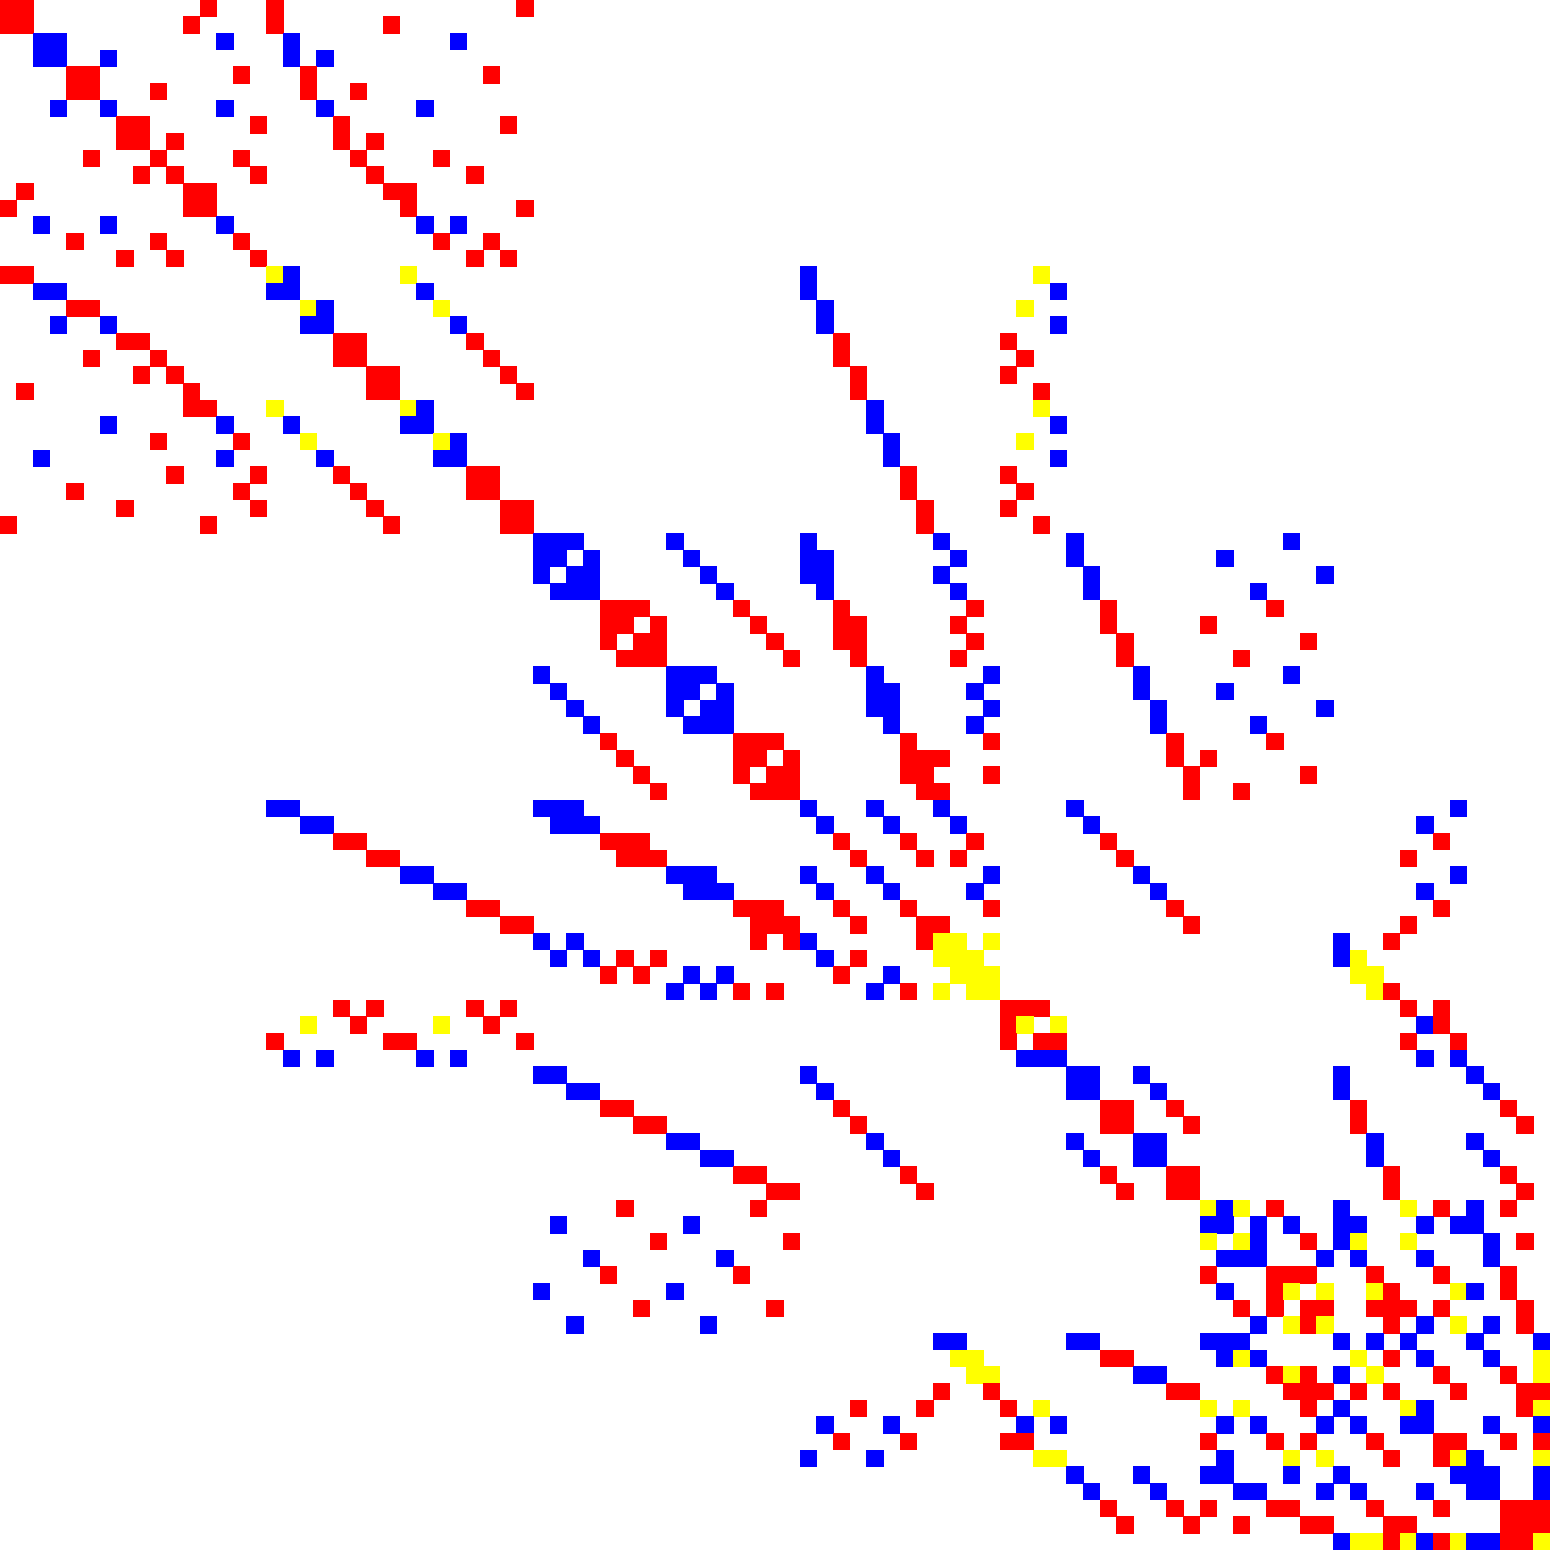
\includegraphics[width=8cm]{cage6.pdf}}
  \caption{Bipartitioning of the $93 \times 93 $ matrix \texttt{cage6} with 785 nonzeros.
The minimum communication volume for an allowed imbalance of $\epsilon=0.03$ equals $V=38$. 
The 397 red nonzeros are assigned to one part, the 316 blue nonzeros to the other part,
and the 72 yellow nonzeros can be freely assigned to any part without affecting
the communication volume, because both their row and their column is already cut.
We can color these free nonzeros to improve the load balance, giving 397 red and 388 blue nonzeros,
corresponding to an achieved imbalance of about $\epsilon^{\prime}=0.01$.}
\end{figure} 

	\section{Acknowledgements}
The computations of this paper on the Dutch national supercomputer Cartesius
at SURFsara in Amsterdam  were carried out under grant
SH-349-15 from The Netherlands Organisation for Scientific Research (NWO).
We thank Oded Schwartz for helpful discussions on \NP-completeness.


	\bibliographystyle{elsarticle-num}
	\bibliography{improved}

\end{document}
